
\usetikzlibrary{arrows.meta,calc,patterns,shapes}
\providecommand{\computer}{%
    
\includegraphics[width=1cm]{../common/Noun_project_216.pdf}
}
\providecommand{\switch}{%
    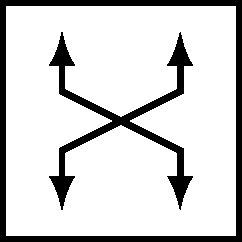
\includegraphics[width=0.9cm]{../common/fig-switch.pdf}
}
\providecommand{\bigswitch}{%
    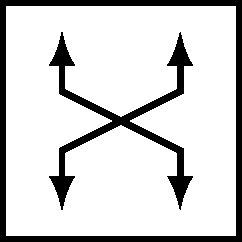
\includegraphics[width=1.4cm]{../common/fig-switch.pdf}
}
\providecommand{\router}{%
    
\includegraphics[width=0.9cm]{../common/fig-router.pdf}
}


\begin{frame}[fragile,label=greSeg]{GRE segment format}
\begin{tikzpicture}
    \tikzset{
        box/.style={draw,thick},
        box unused/.style={draw,thick,pattern=north west lines},
        box label/.style={midway,font=\small,align=center},
        box label flags/.style={midway,font=\fontsize{8}{9}\selectfont,align=center},
        hi on/.style={alt=<#1>{ultra thick,fill=red!10}},
        explain box 1/.style={draw=red,line width=0.8mm,fill=white,anchor=center,at={(explain box loc 1)},align=center},
        explain box 2/.style={draw=red,line width=0.8mm,fill=white,anchor=center,at={(explain box loc 2)},align=center},
        explain box 3/.style={draw=red,line width=0.8mm,fill=white,anchor=center,at={(explain box loc 3)},align=center},
    }
    \begin{scope}[x=4.7mm,y=9mm]
        \coordinate (explain box loc 1) at (16, -3.1);
        \coordinate (explain box loc 2) at (16, -5.1);
        \coordinate (explain box loc 3) at (16, -1.1);
        \path[shading=axis,top color=white,bottom color=black!20] (0, 1) rectangle (32, 0)
            node[box label] {(IP or UDP header (for tunnel))};
        \path[box,hi on=2] (0, 0) rectangle ++(1, -1) node[box label flags] {C};
        \path[box,hi on=0] (1, 0) rectangle ++(1, -1) node[box label flags] {0};
        \path[box,hi on=2] (2, 0) rectangle ++(1, -1) node[box label flags] {K};
        \path[box,hi on=2] (3, 0) rectangle ++(1, -1) node[box label flags] {S};
        \path[box,hi on=0] (4, 0) rectangle (12, -1) node[box label] {0};
        \path[box,hi on=0] (4, 0) rectangle (12, -1) node[box label] {vers\\0};
        \path[box,hi on=0] (16, 0) rectangle (32, -1) node[box label] {protocol type \\ (EtherType)};
        \path[box,hi on=0] (0, -1) rectangle (16, -2) node[box label] {checksum (if C set)};
        \path[box,hi on=0] (16, -1) rectangle (32, -2) node[box label] {0 (if C set)};
        \path[box,hi on=0] (0, -2) rectangle (32, -2) node[box label] {key (if K set)};
        \path[box,hi on=0] (0, -3) rectangle (32, -4) node[box label] {sequence number (if S set)};
        \path[overlay,shading=axis,top color=black!20,bottom color=white] (0, -4) rectangle (32, -5)
            node[box label] {
                encapsulated header+data \\
                (probably IPv4 or IPv6)
            };
        \begin{visibleenv}<2>
            \node[explain box 1] {
                checksum, `key' ($\sim$ port), sequence number optional
            };
        \end{visibleenv}
    \end{scope}
\end{tikzpicture}
\end{frame}
